\begin{figure}

	\centering
	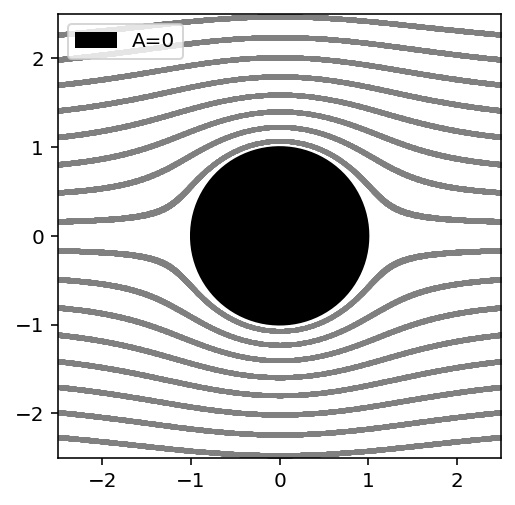
\includegraphics[width=0.45\textwidth]{papers/joukowski/images/05_stroemungslinien/Magnus_Strom_A000_g.png}
	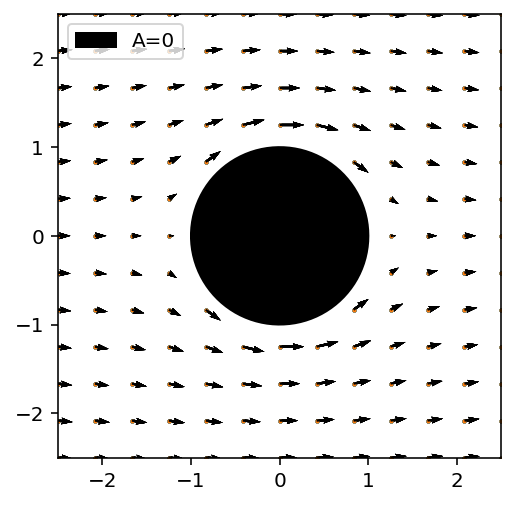
\includegraphics[width = 0.45\textwidth]{papers/joukowski/images/05_stroemungslinien/Magnus_Speed_A000.png}
	\caption{
		Die Strömungslinien werden lokal um das Hindernis des Zylinders gekrümmt,
		dabei nimmt die Geschwindigkeit der Strömung ober- und unterhalb des Zylinders gleichmässig zu.
		\label{joukowski:Stroemungslinien:fig_Zylinder}
	}
\end{figure}
